\chapter{Proposition d'un \textit{Clustering Interactif} pour assister la modélisation d'un jeu de données}
\label{chapter:3-CLUSTERING-INTERACTIF}
	
	% RÉSUMÉ DES ÉPISODES PRÉCÉDENTS: L'ANNOTATION C'EST COMPLIQUÉ !
	Dans le chapitre précédent, nous avons vu les points essentiels suivants :
	%
	\begin{leftBarImportantGreen}
		\begin{todolist}
			% 1. Importance du jeu de données.
			\item[\itemok] Dans un cadre industriel, le choix de l'algorithme utilisé pour l'entraînement d'un modèle est déterminé à l'avance, donc la qualité de l'assistant repose principalement sur la fiabilité et la pertinence de son jeu de données ;
			% 2. Experts métiers avec connaissance métiers, pas de connaissance en datascience.
			\item[\itemok] Pour concevoir ce jeu de données, il est nécessaire de faire appel à des experts maîtrisant le domaine à couvrir par l'assistant car les données sont en général spécifiques ou privées ;
			% 3. Experts métiers ayant peu de donnaissance en data science.
			\item[\itemok] L'intervention de ces experts métiers au sein du projet est en général laborieuse :
			d'une part à cause de leur manque de connaissances en data science (ce n'est pas leur domaine d'expertise),
			d'autre part à cause de la complexité inhérente des tâches de modélisation et d'annotation des données.
			% 4. Tache manuelle avec peu d'assistance.
			\item[\itemok] Par manque de compétences, de connaissances ou d'ergonomie, la tâche de conception d'un jeu de données reste manuelle et est encore mal assistée par ordinateur.
		\end{todolist}
	\end{leftBarImportantGreen}
	\todo[inline]{À REFORMULER APRÈS L'ÉCRITURE DE L'ÉTAT DE L'ART}
	
	% ANNONCE DU BUT DU CHAPITRE: MA CONTRIBUTION !
	Dans cette partie, nous proposons une alternative à l'organisation manuelle destinée à la conception d'un jeu de données.
	Notre proposition vise à remplir un double objectif :
	%
	\begin{leftBarImportantRed}
		\begin{todolist}
			% 1. Efficacité de création du trainset.
			\item Proposer une méthode permettant d'assister la modélisation et l'annotation des données pour créer plus efficacement une base d'apprentissage pour la classification d'intention d'un assistant conversationnel ;
			% 2. Efficacité d'intervention d'un expert.
			\item Redéfinir les tâches et les objectifs des différents acteurs afin de rester au plus proche de leurs compétences réelles, particulièrement en ce qui concerne les experts métiers intervenants dans le projet.
		\end{todolist}
	\end{leftBarImportantRed}

	% TABLE DES MATIÈRES DU CHAPITRE
	\minitoc


	%%%%%--------------------------------------------------------------------
	%%%%% Section 3.1: Intuitions à l'origine.
	%%%%%--------------------------------------------------------------------
	\section{Intuitions à l'origine}
	\label{section:3.1-DESCRIPTION-INTUITIONS}

		% 1. L'annotation de contraintes est plus intuitif pour un expert métier.
		La pierre angulaire de notre méthode repose sur le fait qu'il est difficile pour un expert métier de classer une question suivant une modélisation abstraite prédéfinie :
		cela l'éloigne de ses compétences métiers initiales, nécessite en contre-partie de nombreuses formations, et introduit de nombreuses erreurs d'annotations.
		De fait, il semble plus adéquat de demander à l'expert métier de discriminer deux questions sur la base de leurs réponses :
		une telle approche demande a priori une charge de travail plus faible et semble plus intuitive car elle se rapproche des compétences réelles de l'annotateur (\textguillemets{\textit{est-ce les deux données traite du même cas d'usage ?}}).
		Ainsi, nous basons notre méthode sur l'annotation de contraintes sur les données.
		
		% 2. Un expert métier seul ne peut trouver une modélisation adéquate, il faut se reposer sur l'interaction homme-machine.
		Toutefois, l'annotation de contraintes semble elle aussi fastidieuse.
		En effet, pour faire émerger une base d'apprentissage, il faut annoter un grand nombre de contraintes et être attentifs aux éventuelles incohérences pour ne pas introduire de contraintes contradictoires.
		Pour assister l'expert dans cette tâche, nous avons donc décidé de l'intégrer dans une stratégie d'apprentissage actif en essayant de tirer parti des interactions possibles avec la machine.
		Ce choix est motivé entre autres par l'intuition qu'il est possible de coopérer avec la machine pour obtenir plus efficacement un résultat pertinent.

		% TR:
		C'est sur la combinaison de ces deux éléments que repose notre méthode d'annotation pour concevoir le jeu d'entraînement de notre assistant conversationnel.
		
		% Avantages/Limites: xu-tian:2015:comprehensive-survey-clustering
		% Limite clustering: agarwal-etal:2011:issues-challenges-tools (hyperparamètres) ; steinbach-etal:2004:challenges-clustering-high (high data)
		% Plusieurs types d'interactions possibles : bae-etal:2021:interactive-clustering-comprehensive


	%%%%%--------------------------------------------------------------------
	%%%%% Section 3.2: Description théorique.
	%%%%%--------------------------------------------------------------------
	\section{Description théorique}
	\label{section:3.2-DESCRIPTION-THEORIQUE}
		
		
		%%%
		%%% Subsection 3.2.1. Description générale.
		%%%
		\subsection{Description générale}
		\label{section:3.2.1-DESCRIPTION-THEORIQUE-GENERALE}
		
		% Présentation succinte.
		Nous proposons la méthode suivante pour transformer une collecte de données brutes en une base d'apprentissage nécessaire à l'entraînement d'un assistant conversationnel.
		Cette méthode, que nous appelons \textit{Clustering Interactif} repose principalement sur l'alternance successive entre deux phases clefs (voir \textsc{Figure~\ref{figure:3.2-CLUSTERING-INTERACTIF}}) :
		\begin{itemize}
			\item[\(\bullet\)] une phase d'\textbf{annotation de contraintes}
			par un expert sur la base des connaissances qu'il détient ;
			\item[\(\bullet\)] une phase de \textbf{segmentation automatique} des données
			par une machine sur la base de la proximité sémantique des données et des contraintes précédemment annotées.
		\end{itemize}
		
		% Objectif recherché
		L'objectif recherché en associant ces deux phases est la création d'un cercle vertueux pour améliorer itérativement la qualité de la base d'apprentissage en cours de construction.
		En effet, à chaque itération, l'expert métier obtiendra une proposition de segmentation des données qu'il pourra raffiner pour corriger le fonctionnement de la machine et ainsi obtenir une segmentation plus pertinente à l'itération suivante.
		
		% Figure.
		\begin{figure}[!htb]
			\centering
			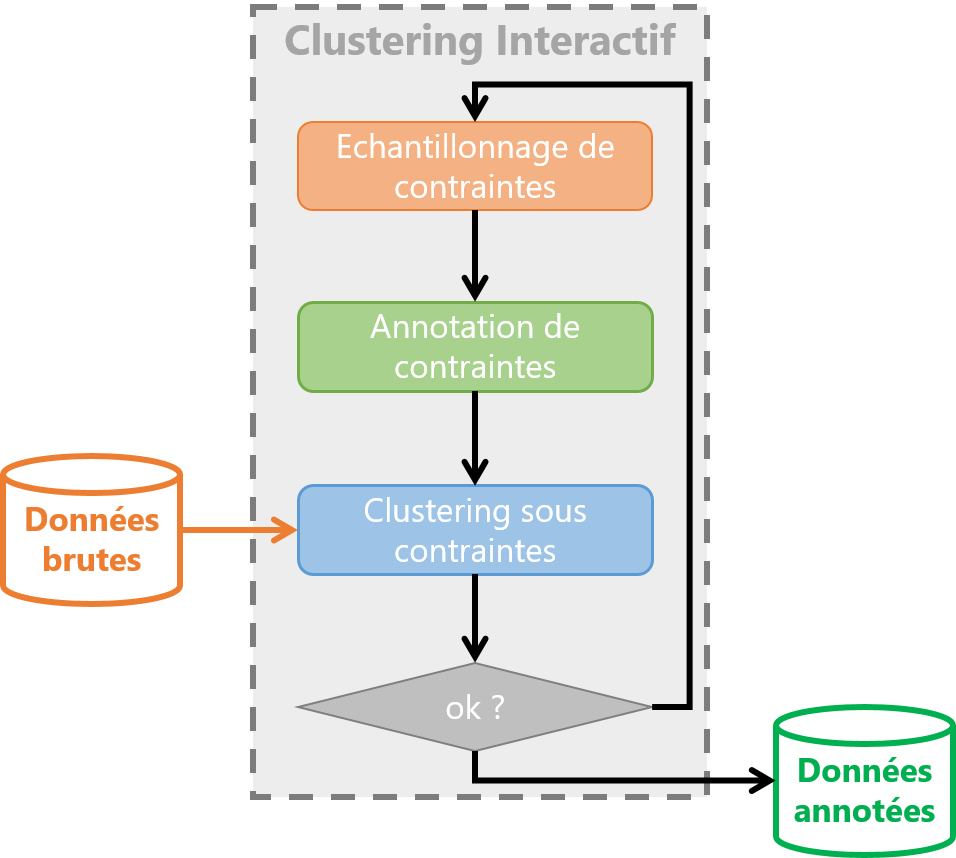
\includegraphics[width=0.95\textwidth]{figures/interactive-clustering-architecture-sequentielle}
			\caption{
				Schéma illustrant l'architecture du \textit{clustering} interactif. La boucle principale enchaîne un échantillonnage de couples de données, une annotation de contraintes, et un \textit{clustering} sous contraintes.
			}
			\label{figure:3.2-CLUSTERING-INTERACTIF}
		\end{figure}
		
		
		%%%
		%%% Subsection 3.2.2. Description détaillée.
		%%%
		\subsection{Description détaillée}
		\label{section:3.2.2-DESCRIPTION-THEORIQUE-DETAILLEE}
		
		% Pseudo code.
		L'\textsc{Algorithme~\ref{algorithm:3.2-CLUSTERING-INTERACTIF}} décrit formellement notre proposition de \textit{Clustering Interactif} que nous détaillons ci-dessous.
		\begin{algorithm}
			\KwData{données non segmentées}
			\KwIn{budget à disposition}
			%
			\textbf{initialisation}: créer une liste vide de contraintes \;
			\textit{optionnel}: évaluer les hyper-paramètres de la segmentation automatique \;
			\textbf{segmentation initial}: regrouper les données par similarité \;
			\Repeat{segmentation satisfaisante OU budget épuisé}{
				\textit{optionnel}: évaluer les hyper-paramètres de l'échantillonnage \;
				\textbf{échantillonnage}: sélectionner une partie de la segmentation à corriger \;
				\textbf{annotation}: corriger la segmentation en ajoutant des contraintes sur l'échantillon \;
				\textit{optionnel}: ré-évaluer les hyper-paramètres de la segmentation automatique \;
				\textbf{segmentation}: regrouper les données par similarité avec les contraintes \;
				\textbf{validation}: estimer la pertinence et la stabilité de la segmentation \;
				\textbf{coûts}: estimer le budget restant et les coûts restant à investir \;
			}
			\textbf{interprétation}: trier et nommer les clusters pour les exploiter \;
			%
			\KwResult{données segmentées (i.e. base d'apprentissage)}
			%
			\caption{\textit{
				Description en pseudo-code de la méthode d'annotation proposée employant le \textit{clustering} interactif.
			}}
			\label{algorithm:3.2-CLUSTERING-INTERACTIF}
		\end{algorithm}
		
		% Description de l'initialisation.
		Pour l'\textbf{initialisation} de la méthode (cf. \textsc{Algorithme~\ref{algorithm:3.2-CLUSTERING-INTERACTIF}}, \textit{lignes 1 à 3}), nous définissons une liste vide de contraintes : tout au long du processus, nous y ajoutons les contraintes annotées par l'expert grâce à ses connaissances métiers (nous entrerons en détails en décrivant la phase d'annotation).
		Il faut aussi une première segmentation des données par la machine : celle-ci se réalise par l'exécution d'un algorithme de \textit{clustering}.
		Nous estimons qu'il n'est pas du ressort de l'expert métier de choisir le réglage de l'algorithme de \textit{clustering} et ses hyper-paramètres.
		Ces derniers pourront être déterminés par un \textit{data scientist} en fonction du problème à traiter ou laissés par défaut.
		Il est à noter que cette première segmentation des données est réalisée sans bénéficier de la connaissance de l'expert, il est donc peu probable que le résultat soit pertinent à ce stade.
		
		% Description de l'échantillonnage.
		Nous entrons dans le coeur de la boucle itérative par la phase d'\textbf{échantillonnage} (cf. \textsc{Algorithme~\ref{algorithm:3.2-CLUSTERING-INTERACTIF}}, \textit{lignes 5 et 6}).
		Comme mentionné au préalable, savoir quelles contraintes ajouter pour corriger efficacement le \textit{clustering} est un problème NP-difficile (le nombre de possibilités croît proportionnellement au carré du nombre de données).
		De plus, l'intervention d'experts est chiffrée et représente en général une partie des coûts à investir dans un projet (voir \textsc{Section~\ref{section:2.3.2.C-DEFIS-ANNOTATION-ASPECT-COMPLEXITE-COUTS}}).
		Il est donc inconcevable de laisser un expert métier annoter des contraintes "seul" et "au hasard".
		Ainsi, pour optimiser ses interventions, il convient de déterminer là où l'expert aura le plus d'impact lors de sa transmission de connaissances.
		C'est pourquoi la phase d'échantillonnage est primordiale dans la méthode proposée : Nous proposons d'y sélectionner des couples de données sur la base de leur similarité, de leur segmentation ou encore de leurs relations avec d'autres données déjà liées par des contraintes.
		
		% Description de l'annotation.
		Sur la base de cet échantillon, l'expert peut entamer son étape d'\textbf{annotation de contraintes} (cf. \textsc{Algorithme~\ref{algorithm:3.2-CLUSTERING-INTERACTIF}}, \textit{ligne 7}).
		Pour alléger la charge d'annotation, nous avons décidé de discriminer les données de l'échantillon par des contraintes binaires simples : \texttt{MUST-LINK} et \texttt{CANNOT-LINK}. Ces contraintes représentent respectivement la similitude ou la différence entre deux données, et seront utilisées pour regrouper ou séparer certaines données dans la prochaine segmentation.
		En fonction de l'orientation du projet et afin de rester au plus proche des compétences réelles de l'expert, la formulation de l'énoncer d'annotation doit être judicieusement définie : par exemple, les contraintes peuvent représenter une similitude
		sur la thématique concernée\footnote{
			Exemples de thématiques : \textit{crédit} vs. \textit{assurance} ; \textit{sport} vs. \textit{culture}, ...
		}, sur l'action désirée\footnote{
			Exemples d'actions : \textit{souscrire} vs. \textit{résilier} ; \textit{activer} vs. \textit{désactiver} ; \textit{s'informer} vs. \textit{réaliser}, ...
		}, ou encore sur le besoin de l'utilisateur\footnote{
			Exemple de besoins : \textit{souscrire un crédit} vs. \textit{souscrire une assurance} ; \textit{s'informer en sport} vs. \textit{s'informer en culture}, ...
		}.
		On notera que des incohérences peuvent s'introduire, ayant pour conclusions de devoir à la fois considérer comme similaires et différentes deux données (voir la gestion des conflits en \textsc{Section~\ref{section:3.3.2-GESTION-DES-CONTRAINTES}}).
		
		% Description du clustering.
		Pour finir, la dernière phase de cette boucle est composée d'une nouvelle \textbf{segmentation} des données (cf. \textsc{Algorithme~\ref{algorithm:3.2-CLUSTERING-INTERACTIF}}, \textit{lignes 8 et 9}).
		Cette segmentation devra respecter les contraintes préalablement définies par l'expert, nous nous tournons donc vers l'utilisation d'un \textit{clustering} sous contraintes.
		Au fur et à mesure des itérations, de plus en plus de contraintes seront ajoutées pour corriger le \textit{clustering}. ainsi, au bout d'un certain nombre d'itérations, la segmentation des données reflétera la vision que l'expert aura voulu transmettre.
		Comme précédemment, nous estimons qu'il n'est pas du ressort de l'expert métier de choisir de l'algorithme de \textit{clustering} et ses hyper-paramètres.
		Ces derniers pourront être déterminés par un \textit{data scientist} en fonction du problème à traiter, estimés en fonction de l'itération et des contraintes disponibles, ou laissés par défaut.
		
		% Description de l'évaluation.
		Comme la méthode est itérative, il faut pouvoir estimer des \textbf{cas d'arrêt} (cf. \textsc{Algorithme~\ref{algorithm:3.2-CLUSTERING-INTERACTIF}}, \textit{lignes 10 à 12}).
		Le cas d'arrêt le plus évident n'est pas technique mais relatif aux coûts investis dans l'opération : si le projet n'a plus de budget dédié à l'annotation, il faudra créer la base d'apprentissage avec le résultat à disposition, quel que soit la pertinence de la segmentation obtenue sur les données.
		Ce cas d'arrêt par défaut peut malheureusement être synonyme d'échec pour le projet si les résultats sont inexploitables.
		D'autres cas d'arrêts peuvent être envisagés en fonction de la qualité ou de la pertinence de la segmentation.
		D'une part, nous pouvons comparer l'évolution de la segmentation des données : si les segmentations sont similaires sur plusieurs itérations, il est possible que la modélisation atteint un optimum local ou un palier de performance.
		D'autre part, nous pouvons aussi comparer l'évolution de l'accord entre la segmentation obtenue et l'annotation de l'expert : en effet, si l'expert ne contredit plus la répartition proposée des données, il est probable que sa vision et la vision de la machine aient convergé.
		Dans les deux cas, l'analyse de l'expert métier reste nécessaire pour valider si la modélisation des données est pertinente ou si elle comporte encore des incohérences à corriger.

		% Description de l'évaluation.
		Lorsque la boucle itérative est finie, nous avons à disposition une segmentation des données qui a été corrigé par un expert et qui reflète ses connaissances métier.
		La dernière étape consiste alors à \textbf{interpréter} ces \textit{clusters} pour pouvoir les exploiter (cf. \textsc{Algorithme~\ref{algorithm:3.2-CLUSTERING-INTERACTIF}}, \textit{ligne 13}).
		Cela commence par leur attribuer un nom au lieu de leur identifiant technique, de les définir en les rapprochant d'un cas d'usage métier, et éventuellement de les raffiner manuellement en supprimant certaines données aberrantes.
		
		
	%%%%%--------------------------------------------------------------------
	%%%%% Section 3.3: Description technique et implémentation.
	%%%%%--------------------------------------------------------------------
	\section{Description technique et implémentation}
	\label{section:3.3-DESCRIPTION-IMPLEMENTATION}
		
		% Généralités.
		Nous avons réalisé une implémentation en Python de notre \textit{clustering interactif}. Celle-ci est répartie en trois librairies :
		\begin{enumerate}
			\item \texttt{cognitivefactory-interactive-clustering}, regroupant les gestions de données, de contraintes et les algorithmes de \textit{Machine Learning} qui ont été implémentés ;
			\item \texttt{cognitivefactory-features-maximization-metrics}, disposant d'une méthode de sélection des patterns linguistiques pertinents (composantes principales) d'un jeu de données ;
			\item \texttt{cognitivefactory-interactive-clustering-gui}, encapsulant les algorithmes précédents et intégrant la logique de la méthode dans une interface graphique.
		\end{enumerate}
		
		% Exemple.
		Pour les sections suivantes, nous suivrons l'exemple suivant (cf. \textsc{Code~\ref{code:3.3-IMPLEMENTATION-DATA}}) pour présenter nos implémentations.
		
		\begin{lstlisting}[
			language=Python,
			caption={Jeu exemple pour présenter notre implémentation du \textit{clustering} interactif.},
			label={code:3.3-IMPLEMENTATION-DATA},
		]
# Définir les données.
dict_of_texts = {
	"0": "Comment signaler un vol de carte bancaire ?",
	"1": "J'ai égaré ma carte bancaire, que faire ?",
	"2": "J'ai perdu ma carte de paiement",
	"3": "Le distributeur a avalé ma carte !",
	"4": "En retirant de l'argent, le GAB a gardé ma carte...",
	"5": "Le distributeur ne m'a pas rendu ma carte bleue.",
	# ...
	"N": "Pourquoi le sans contact ne fonctionne pas ?",
}
		\end{lstlisting}
		
		
		%%%
		%%% Subsection 3.3.1: Gestion des données.
		%%%
		\subsection{Gestion des données}
		\label{section:3.3.1-GESTION-DES-DONNEES}
				
		% cognitivefactory.interactive-clustering.utils
		Tout d'abord, en ce qui concerne la \textbf{manipulation de données}, nous utilisons le module \texttt{utils} de la librairie \texttt{cognitivefactory-interactive-clustering}.
		Les données sont stockées dans un dictionnaire Python afin de tracer les manipulations à l'aide d'une clé servant d'identifiant de la donnée.
		
		% cognitivefactory.interactive-clustering.utils.preprocessing : Implémentation.
		Nous avons d'une part la partie \texttt{utils.preprocessing}\footnote{
			\texttt{utils.preprocessing}: \url{https://cognitivefactory.github.io/interactive-clustering/reference/cognitivefactory/interactive_clustering/utils/preprocessing/}
		} qui permet de normaliser les données.
		Par défaut :
		\begin{itemize}
			\item[\(\bullet\)] le texte est passé en \textit{minuscule} (de "\texttt{Bonjour}" à "\texttt{bonjour}"),
			\item[\(\bullet\)] la \textit{ponctuation} est supprimée, %(\texttt{.}, \texttt{,}, \texttt{;}, \texttt{:}, \texttt{!}, \texttt{¡}, \texttt{?}, \texttt{¿}, \texttt{…}, \texttt{•}, \texttt{(}, \texttt{)}, \texttt{\{}, \texttt{\}}, \texttt{[}, \texttt{]}, \texttt{\textguillemets{}, \texttt{}}, \texttt{^}, \texttt{\`}, \texttt{'}, \texttt{"}, \texttt{\\}, \texttt{/}, \texttt{|}, \texttt{-}, \texttt{\_}, \texttt{#}, \texttt{\&}, \texttt{\~}, \texttt{\@}),
			\item[\(\bullet\)] les \textit{accents} sont enlevés (de "\texttt{crédit}" à "\texttt{credit}"),
			\item[\(\bullet\)] et les multiples \textit{espaces blancs} sont convertis en un unique espace simple (de "\texttt{au~~~~revoir}" à "\texttt{au revoir}").
		\end{itemize}
		
		Si besoin, trois options "avancées" sont disponibles pour réaliser un prétraitement plus destructif :
		\begin{itemize}
			\item[\(\bullet\)] la suppression des mots vides (\cite{nothman-etal:2018:stop-word-lists}),
			\item[\(\bullet\)] la conversion des mots vers leur forme racine (\cite{manning-schutze:2000:foundations-statistical-natural}),
			\item[\(\bullet\)] et la suppression des mots en fonction de leur profondeur dans l'arbre de dépendance syntaxique (\cite{nivre:2006:inductive-dependency-parsing}).
		\end{itemize}
		
		% cognitivefactory.interactive-clustering.utils.preprocessing : Dépendances.
		Ces traitements sont réalisés en bénéficiant des fonctionnalités mises à disposition d'un modèle de langue de type SpaCy (\cite{honnibal-montani:2017:spacy-natural-language}), avec par défaut l'utilisation du modèle \texttt{fr-core-news-md}.
		
		% cognitivefactory.interactive-clustering.utils.preprocessing : Par défaut.
		Pour nos études, nous définissons quatre niveaux de prétraitements facilement identifiables :
		\begin{enumerate}
			\item L'\textbf{absence de prétraitement}, soit la conservation de la donnée brute, noté \texttt{prep.no} ;
			\item Le \textbf{prétraitement simple}, correspondant au traitement traitement de base (minuscules, ponctuations, accents, espaces blancs), noté \texttt{prep.simple} ; 
			\item Le \textbf{prétraitement lemmatisé}, correspondant au traitement de base auquel s'ajoute la lemmatisation des mots, noté \texttt{prep.lemma} ;
			\item le \textbf{prétraitement avec filtres}, correspondant au traitement de base avec l'élagage de l'arbre de dépendance syntaxique de la phrase, noté \texttt{prep.filter}.
		\end{enumerate}
		
		
		% cognitivefactory.interactive-clustering.utils.vectorization
		D'autre part, la partie \texttt{utils.vectorization}\footnote{
			\texttt{utils.vectorization}: \url{https://cognitivefactory.github.io/interactive-clustering/reference/cognitivefactory/interactive_clustering/utils/vectorization/}
		} permet de transformer les données en une représentation exploitable pour la machine.
		Deux modes de vectorisation sont mis à disposition :
		\begin{enumerate}
			\item \textbf{TF-IDF} (\cite{ramos:2003:using-tfidf-determine}), utilisant la fréquence d'occurrence des mots pour représenter une phrase, et noté \texttt{vect.tfidf} pour nos études ;
			\item \textbf{SpaCy} (\cite{honnibal-montani:2017:spacy-natural-language}), utilisant le modèle de langue \texttt{fr-core-news-md}, et noté \texttt{vect.frcorenewsmd}.
		\end{enumerate}
		
		% cognitivefactory.interactive-clustering.utils : Exemple.
		Vous avez un exemple d'utilisation des modules de prétraitements et de vectorisation dans \textsc{Code~\ref{code:3.3-IMPLEMENTATION-GESTION-DONNEES}}.
		
		\begin{lstlisting}[
			language=Python,
			caption={Démonstration de notre implémentation du prétraitement et de la vectorisation sur le jeu d'exemple.},
			label={code:3.3-IMPLEMENTATION-GESTION-DONNEES},
		]
# Import des dépendances.
from cognitivefactory.interactive_clustering.utils.preprocessing import preprocess
from cognitivefactory.interactive_clustering.utils.vectorization import vectorize

# Prétraitement des données.
dict_of_preprocess_texts = preprocess(
	dict_of_texts=dict_of_texts,
	apply_stopwords_deletion=False,
	apply_parsing_filter=False,
	apply_lemmatization=False,
	spacy_language_model="fr_core_news_md",
)
"""
	{"0": "comment signaler un vol de carte bancaire",
	 "1": "j ai egare ma carte bancaire, que faire",
	 "2": "j ai perdu ma carte de paiement",
	 "3": "le distributeur a avale ma carte",
	 "4": "en retirant de l argent le gab a garde ma carte",
	 "5": "le distributeur ne m a pas rendu ma carte bleue",
	 # ...
	 "N": "pourquoi le sans contact ne fonctionne pas"}
"""

# Vectorisation des données.
dict_of_vectors = vectorize(
	dict_of_texts=dict_of_preprocess_texts,
	vectorizer_type="tfidf",
)
		\end{lstlisting}
		
		%%%
		%%% Subsection 3.3.2: Gestion des contraintes
		%%%
		\subsection{Gestion des contraintes}
		\label{section:3.3.2-GESTION-DES-CONTRAINTES}
		
		% cognitivefactory.interactive-clustering.constraints
		En ce qui concerne la \textbf{manipulation de contraintes}, nous utilisons le module \texttt{contraints}\footnote{
			\texttt{constraints}: \url{https://cognitivefactory.github.io/interactive-clustering/reference/cognitivefactory/interactive_clustering/constraints/}
		} de la librairie \texttt{cognitivefactory-interactive-clustering}.
		
		% cognitivefactory.interactive-clustering.constraints: Types
		Deux types de contraintes sont prises en charge (cf.~\cite{wagstaff-cardie:2000:clustering-instancelevel-constraints}) :
		\begin{itemize}
			\item[\(\bullet\)] les contraintes \texttt{MUST-LINK} permettant de réunir deux données,
			\item[\(\bullet\)] et les contraintes \texttt{CANNOT-LINK} permettant à l'inverse de les séparer.
		\end{itemize}

		% cognitivefactory.interactive-clustering.constraints: Transitivité.
		Ces types de contraintes respectent les propriétés de transitivités décrites dans l'\textsc{Equation~\ref{equation:3.3-CONTRAINTES-TRANSITIVITE}}) et sont illustrées dans la \textsc{Figure~\ref{figure:3.3-CONTRAINTES-TRANSITIVITE}} (\textbf{(1)} et \textbf{(2)}).
		On note ainsi qu'il est possible de déduire la troisième contrainte d'un triangle de trois points si nous connaissons déjà les deux premières.
		
		\begin{equation}
			\label{equation:3.3-CONTRAINTES-TRANSITIVITE}
			(\forall A,B,C)~
			\begin{cases}
				% ML + ML => ML
				~\textcolor{colorDarkPastelGreen}{\texttt{MUST\_LINK}}(A,B)
				~\wedge~\textcolor{colorDarkPastelGreen}{\texttt{MUST\_LINK}}(B,C)
				~\Rightarrow~\textcolor{colorDarkPastelGreen}{\texttt{MUST\_LINK}}(A,C)  \\
				% ML + CL => CL
				~\textcolor{colorDarkPastelGreen}{\texttt{MUST\_LINK}}(A,B)
				~\wedge~\textcolor{colorDarkPastelRed}{\texttt{CANNOT\_LINK}}(B,C)
				~\Rightarrow~\textcolor{colorDarkPastelRed}{\texttt{CANNOT\_LINK}}(A,C)
			\end{cases}
		\end{equation}
		
		Pour respecter ces propriétés, le gestionnaire de contraintes doit ainsi calculer les transitivités à chaque ajout ou suppression de contraintes.
		On distinguera donc une contrainte ajoutée (\texttt{added}) d'une contrainte déduite par transitivité (\texttt{inferred}).
		
		% cognitivefactory.interactive-clustering.constraints: Conflits.
		Il se peut que la contrainte en cours d'ajout contredise les contraintes précédemment déduites : nous parlons alors d'incohérence ou de conflit (cf. \textsc{Figure~\ref{figure:3.3-CONTRAINTES-TRANSITIVITE}} et \textsc{Equation~\ref{equation:3.3-CONTRAINTES-CONFLITS}}).
		Dans ce cas, l'ajout de la dernière contrainte n'est pas prise en compte et le gestionnaire renvoie une erreur permettant d'identifier ce conflit.
		Ce conflit peut venir simplement venir d'une erreur d'inattention, mais peut aussi venir d'une déduction basée sur des ajouts antérieurs erronés.
		Sémantiquement, un conflit indique une contradiction dans la gestion des données, car les données concernées doivent à la fois être réunies et séparées...
		
		\begin{equation}
			\label{equation:3.3-CONTRAINTES-CONFLITS}
			(\exists A,B,C)~
			~\textcolor{colorDarkPastelGreen}{\texttt{MUST\_LINK}}(A,B)
			~\wedge~\textcolor{colorDarkPastelGreen}{\texttt{MUST\_LINK}}(B,C)
			~\wedge~\textcolor{colorDarkPastelRed}{\texttt{CANNOT\_LINK}}(A,C)
		\end{equation}
		
		% cognitivefactory.interactive-clustering.constraints: Composants connexe.
		À partir d'une donnée \(D\), et par application de la propriété de transitivité des \texttt{MUST-LINK}, nous appelons \textbf{composant connexe} de \(D\) l'ensemble des données \(D_i\) liées par une succession de contraintes \texttt{MUST-LINK} à \(D\) (cf. \textsc{Figure~\ref{figure:3.3-CONTRAINTES-TRANSITIVITE}}).
		Ce composant peut être vu comme un noyau de \textit{cluster}.
		Il pourra être associé à d'autres noyaux par similarité pour former un \textit{cluster} plus conséquent, ou être distingué d'autres noyaux pour former plusieurs \textit{clusters}.

		\begin{figure}[!htb]
			\centering
			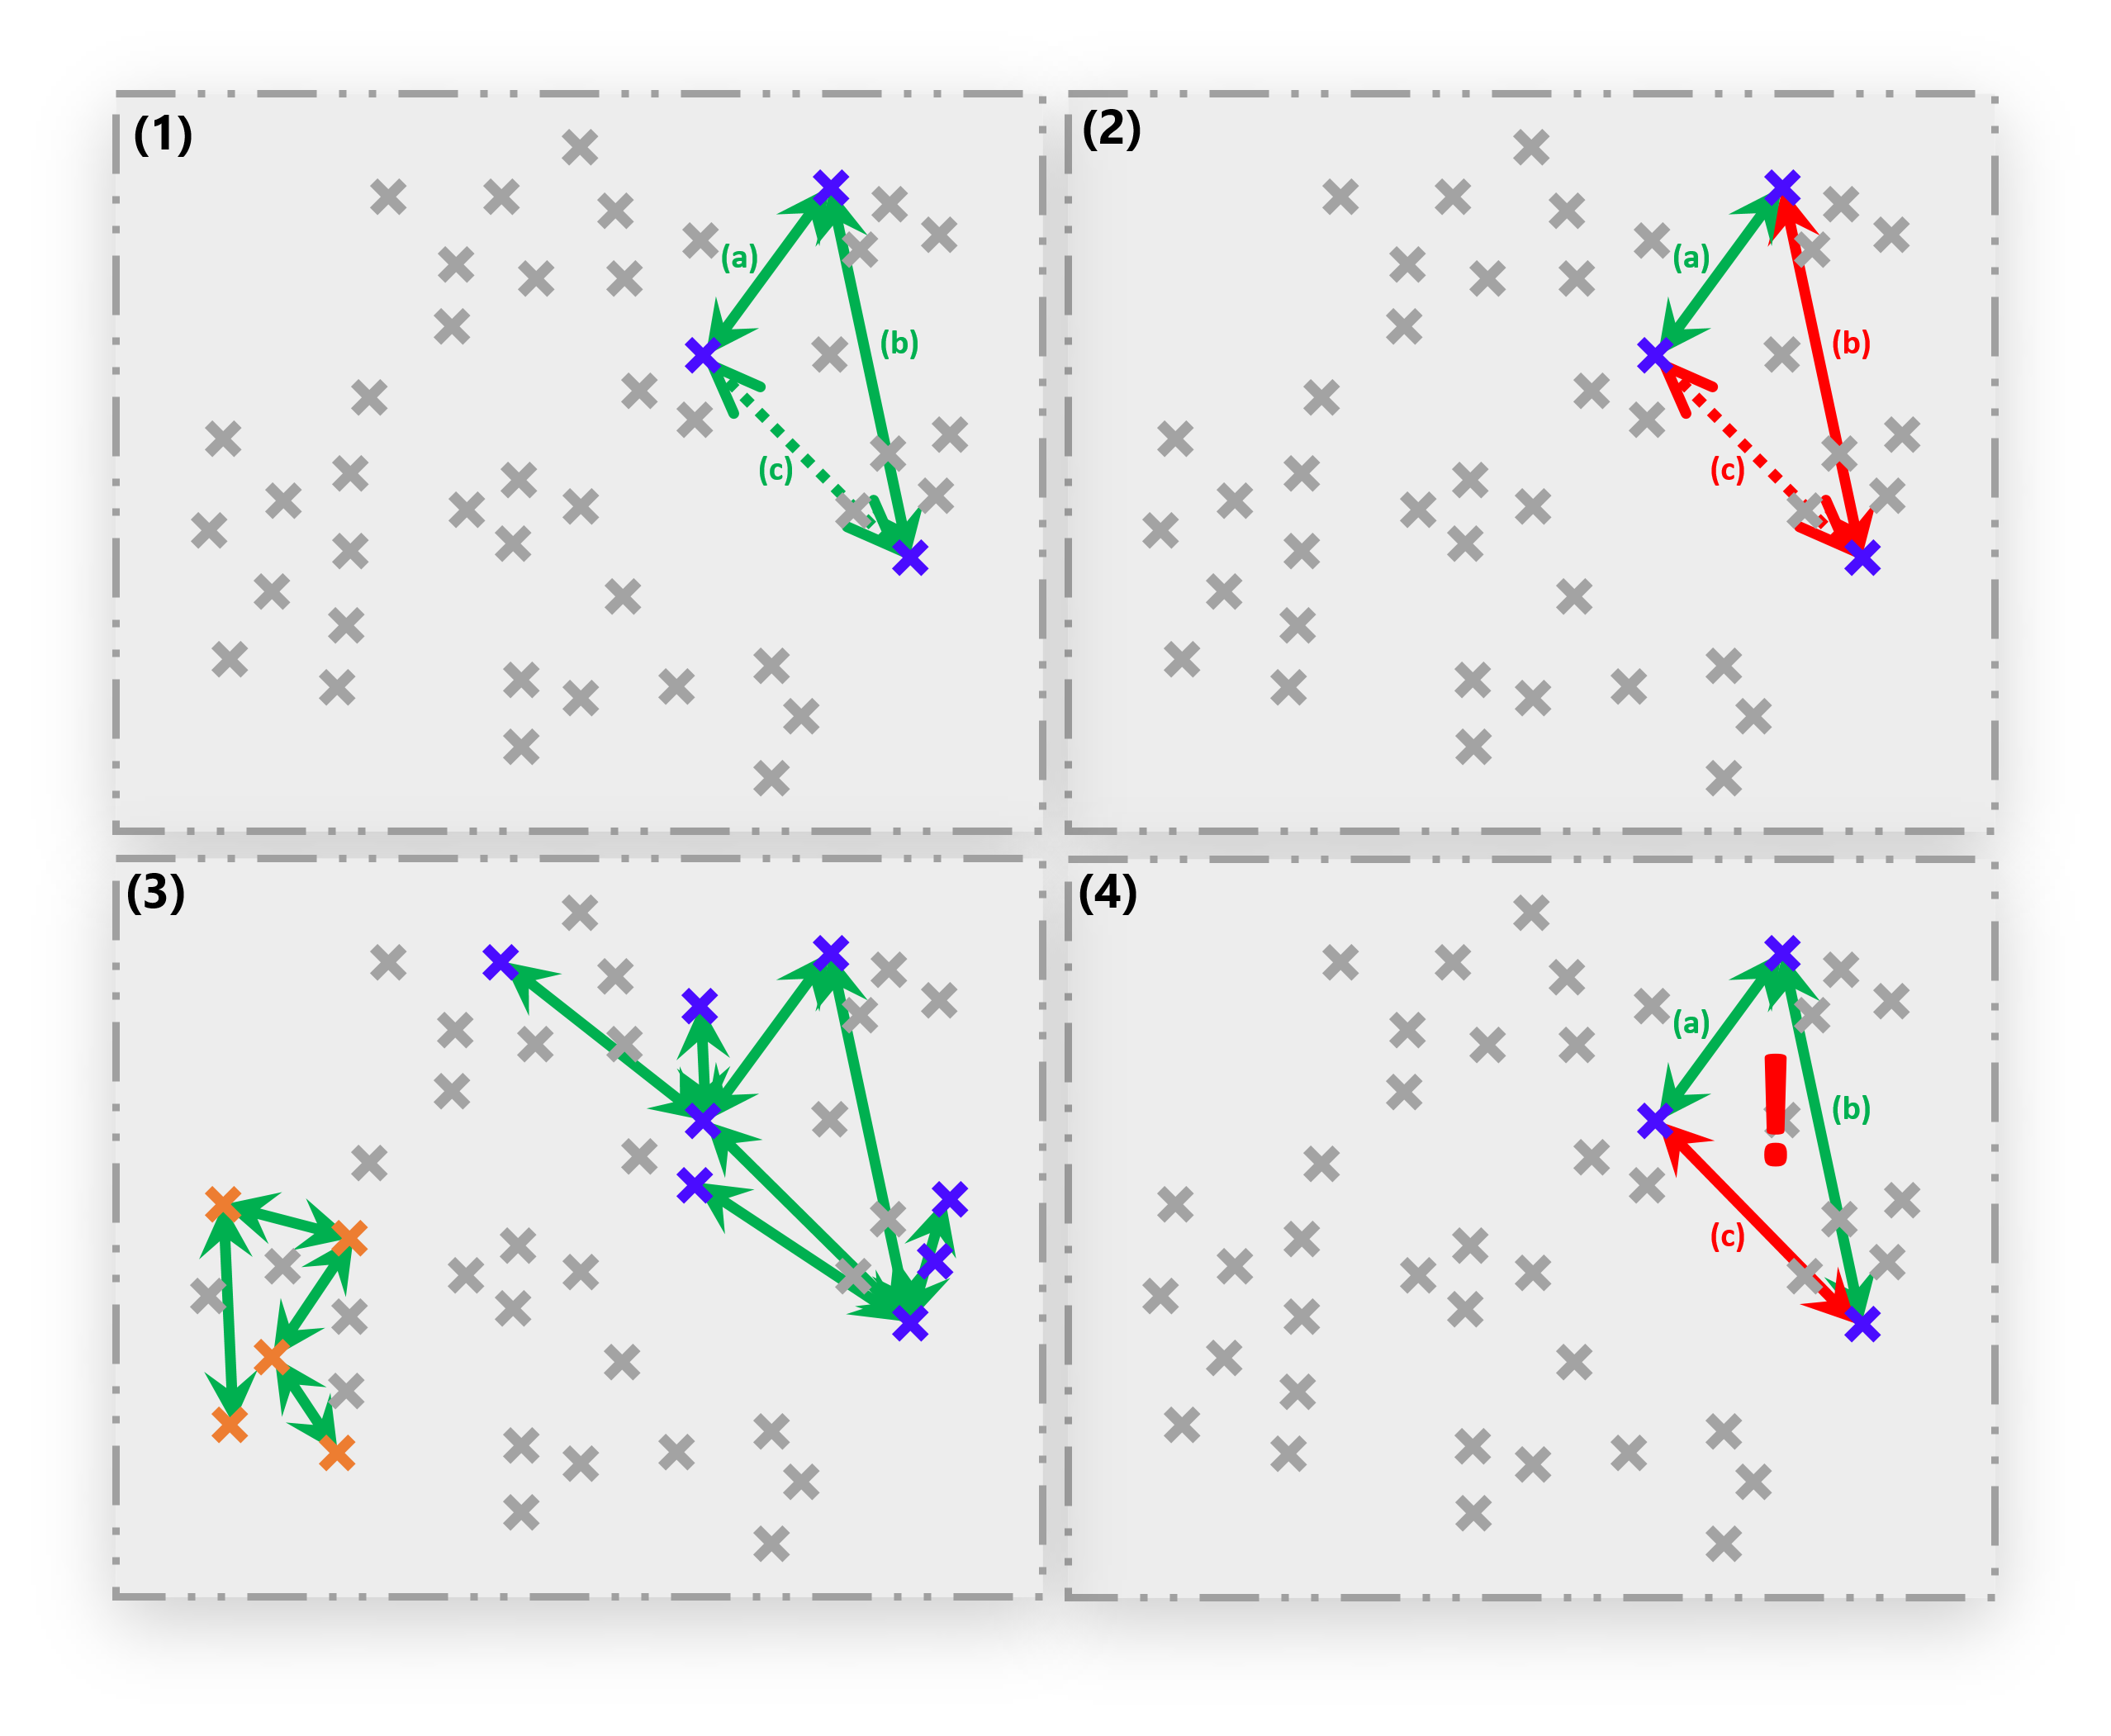
\includegraphics[width=0.70\textwidth]{figures/example-constraints-transitivity}
			\caption{
				Exemples des propriétés de transitivité des contraintes \texttt{MUST-LINK} (flèches vertes) et \texttt{CANNOT-LINK} (flèches rouges). \textbf{(1)} et \textbf{(2)} représente les possibilités de déduction d'une contrainte (\texttt{(c)}) en fonction des deux autres (\texttt{(a)} et \texttt{(b)}). \textbf{(3)} représente deux composants connexes définis par la transitivité des contraintes \texttt{MUST-LINK}. Enfin, \textbf{(4)} représente un cas de conflit où une contrainte (\texttt{(c)}) ne correspond pas à sa déduction faite à partir des autres contraintes (\texttt{(a)} et \texttt{(b)}).
			}
			\label{figure:3.3-CONTRAINTES-TRANSITIVITE}
		\end{figure}
		
		% cognitivefactory.interactive-clustering.constraints : Exemple.
		Un exemple d'utilisation du module de gestion de contraintes est consultable dans \textsc{Code~\ref{code:3.3-IMPLEMENTATION-GESTION-CONTRAINTES}}.
		
		\begin{lstlisting}[
			language=Python,
			caption={Démonstration de notre implémentation de gestion des contraintes sur le jeu d'exemple.},
			label={code:3.3-IMPLEMENTATION-GESTION-CONTRAINTES},
		]
# Import des dépendances.
from cognitivefactory.interactive_clustering.constraints.factory import managing_factory

# Création du gestionnaire de contraintes.
constraints_manager = managing_factory(
	manager="binary",
	list_of_data_IDs = list(dict_of_texts.keys()),  # ["0", "1", "2", "3", "4", "5", ..., "N"]
)

# Ajout de contraintes.
constraints_manager.add_constraint(
	data_ID1="0",  # "Comment signaler un vol de carte bancaire ?"
	data_ID2="1",  # "J'ai égaré ma carte bancaire, que faire ?"
	constraint_type="MUST_LINK",
)
constraints_manager.add_constraint(
	data_ID1="3",  # "Le distributeur a avalé ma carte !"
	data_ID2="4",  # "En retirant de l'argent, le GAB a gardé ma carte..."
	constraint_type="MUST_LINK",
)
constraints_manager.add_constraint(
	data_ID1="0",  # "Comment signaler un vol de carte bancaire ?"
	data_ID2="N",  # "Pourquoi le sans contact ne fonctionne pas ?"
	constraint_type="CANNOT_LINK",
)
	# NB: ajouter une contrainte "MUST_LINK" entre "1" et "N" lèverait une erreur.

# Récupération des composants connexes.
connected_components = constraints_manager.get_connected_components()
"""
	[['0', '1'],
	 ['2'],
	 ['3', '4'],
	 ['5'],
	 ['N']]
"""
		\end{lstlisting}
		
		
		%%%
		%%% Subsection 3.3.3: Algorithme de \textit{clustering} sous contraintes.
		%%%
		\subsection{Algorithme de \textit{clustering} sous contraintes}
		\label{section:3.3.3-ALGORITHMES-CLUSTERING-SOUS-CONTRAINTES}
		
		% cognitivefactory.interactive-clustering.clustering
		En ce qui concerne le \textbf{regroupement automatique} des données par similarité, nous utilisons le module \texttt{clustering}\footnote{
			\texttt{clustering}: \url{https://cognitivefactory.github.io/interactive-clustering/reference/cognitivefactory/interactive_clustering/clustering/}
		} de la librairie \texttt{cognitivefactory-interactive-clustering}.
		
		% cognitivefactory.interactive-clustering.utils.clustering : Implémentation.
		Ce module met à disposition six algorithmes de \textit{clustering} sous contraintes :
		\begin{enumerate}
			\item \textbf{KMeans}, dans sa version \texttt{COP} (\cite{wagstaff-etal:2001:constrained-kmeans-clustering}), noté \texttt{clust.kmeans.cop}, et sa version \texttt{MPC} (\cite{khan-etal:2012:multiple-parameter-based}), noté \texttt{clust.kmeans.mpc}) ;
			\item \textbf{DBscan}, dans sa version \texttt{C-DBScan} (\cite{ruiz-etal:2010:densitybased-semisupervised-clustering}), noté \texttt{clust.cdbscan} ;
			\item \textbf{Hiérarchique} (\cite{davidson-ravi:2005:agglomerative-hierarchical-clustering}), avec quatre métriques de distances : \textit{single} (noté \texttt{clust.hier.sing}), \textit{complete} (noté \texttt{clust.hier.comp}), \textit{average} (noté \texttt{clust.hier.avg}) et \textit{ward} (noté \texttt{clust.hier.ward}) ;
			\item \textbf{Spectral}, dans sa version \texttt{SPEC} (\cite{kamvar-etal:2003:spectral-learning}), noté \texttt{clust.spec} ;
			\item \textbf{Propagation par affinité} (\cite{givoni-frey:2009:semisupervised-affinity-propagation}), noté \texttt{clust.affprop}.
		\end{enumerate}
		
		Une classe abstraite définit les prérequis des algorithmes implémentés (avoir une méthode \texttt{cluster}) et une \textit{factory} est disponible pour instancier rapidement un objet de \textit{clustering}.
		% cognitivefactory.interactive-clustering.clustering : Exemple.
		Enfin, un exemple d'utilisation ce module est consultable dans \textsc{Code~\ref{code:3.3-IMPLEMENTATION-CLUSTERING}}.
		
		
		\begin{lstlisting}[
			language=Python,
			caption={Démonstration de notre implémentation du \textit{clustering} sous contraintes sur le jeu d'exemple.},
			label={code:3.3-IMPLEMENTATION-CLUSTERING},
		]
# Import des dépendances.
from cognitivefactory.interactive_clustering.clustering.factory import clustering_factory

# Initialiser un objet de clustering.
clustering_model = clustering_factory(
	algorithm="kmeans",
	model="COP",
	random_seed=42,
)

# Lancer le clustering.
clustering_result = clustering_model.cluster(
	constraints_manager=constraints_manager,  # contient les contraintes
	nb_clusters=2,
	vectors=dict_of_vectors,
)
"""
	{"0": 0,  # "Comment signaler un vol de carte bancaire ?"
	 "1": 0,  # "J'ai égaré ma carte bancaire, que faire ?"
	 "2": 0,  # "J'ai perdu ma carte de paiement"
	 "3": 1,  # "Le distributeur a avalé ma carte !"
	 "4": 1,  # "En retirant de l'argent, le GAB a gardé ma carte..."
	 "5": 1,  # "Le distributeur ne m'a pas rendu ma carte bleue."
	 # ...
	 "N": 1}  # "Pourquoi le sans contact ne fonctionne pas ?"
"""
		\end{lstlisting}
		
		% cognitivefactory.interactive-clustering.utils.clustering : Historique.
		\begin{leftBarInformation}
			Dans le cadre d'un projet étudiant avec l'école d'ingénieur Télécom Physique Strasbourg, les implémentations des algorithmes  KMeans (\texttt{MPC}), C-DBScan et propagation par affinité ont été ajoutées. Les élèves ont conclu ce projet d'extension en suggérant de se concentrer sur l'étude du C-DBScan car les deux autres algorithmes étaient soit trop instables, soit trop gourmand en temps de calcul.
			Les autres algorithmes (KMeans (\texttt{COP}), hiérarchique et spectral (\texttt{SPEC})) ont été implémentés au début de ce doctorat.
		\end{leftBarInformation}
		
		
		%%%
		%%% Subsection 3.3.4: Algorithme d'échantillonnage de contraintes.
		%%%
		\subsection{Algorithme d'échantillonnage de contraintes}
		\label{section:3.3.4-ALGORITHMES-ECHANTILLONNAGE-DE-CONTRAINTES}
		
		% cognitivefactory.interactive-clustering.sampling
		En ce qui concerne l'\textbf{échantillonnage} de contraintes à annoter, nous utilisons le module \texttt{sampling}\footnote{
			\texttt{sampling}: \url{https://cognitivefactory.github.io/interactive-clustering/reference/cognitivefactory/interactive_clustering/sampling/}
		} de la librairie \texttt{cognitivefactory-interactive-clustering}.
		
		% cognitivefactory.interactive-clustering.utils.sampling : Implémentation.
		Cet échantillonnage correspond à la sélection de couple de données.
		Par défaut, l'échantillonnage est purement aléatoire.
		Cependant, plusieurs options sont disponibles :
		
		\begin{itemize}
			\item[\(\bullet\)] une restriction sur la \textit{distance} pouvant imposer aux données d'être les plus proches ou les plus éloignées du corpus ;
			\item[\(\bullet\)] une restriction sur le \textit{résultat du clustering} pouvant imposer aux données d'être issues d'un même cluster ou de clusters différents,
			\item[\(\bullet\)] une restriction pour exclure les contraintes \textit{déjà annotées},
			\item[\(\bullet\)] et enfin une restriction pour exclure les contraintes \textit{déjà déduites} par transitivité.
		\end{itemize}
		
		% cognitivefactory.interactive-clustering.utils.sampling : Par défaut.
		Sur cette base, nous définissons quatre niveaux d'échantillonnage facilement identifiables pour nos études :
		\begin{enumerate}
			\item Un échantillonnage \textbf{purement aléatoire} en excluant toutes les contraintes déjà annotées ou déduites, noté \texttt{samp.random.full} ;
			\item Un échantillonnage \textbf{pseudo-aléatoire} de données issues d'un \textbf{même cluster}, en excluant toutes les contraintes déjà annotées ou déduites, noté \texttt{samp.random.same} ;
			\item Un échantillonnage des données issues d'un \textbf{même cluster} et étant \textbf{les plus éloignées} les unes des autres, noté \texttt{samp.farhtest.same} (cf. \textsc{Figure~\ref{figure:3.3-CONTRAINTES-SAMPLING}}) ;
			\item Un échantillonnage des données issues de \textbf{clusters différents} et étant \textbf{les plus proches} les unes des autres, noté \texttt{samp.closest.diff} (cf. \textsc{Figure~\ref{figure:3.3-CONTRAINTES-SAMPLING}}).
		\end{enumerate}
		
		\begin{figure}[!htb]
			\centering
			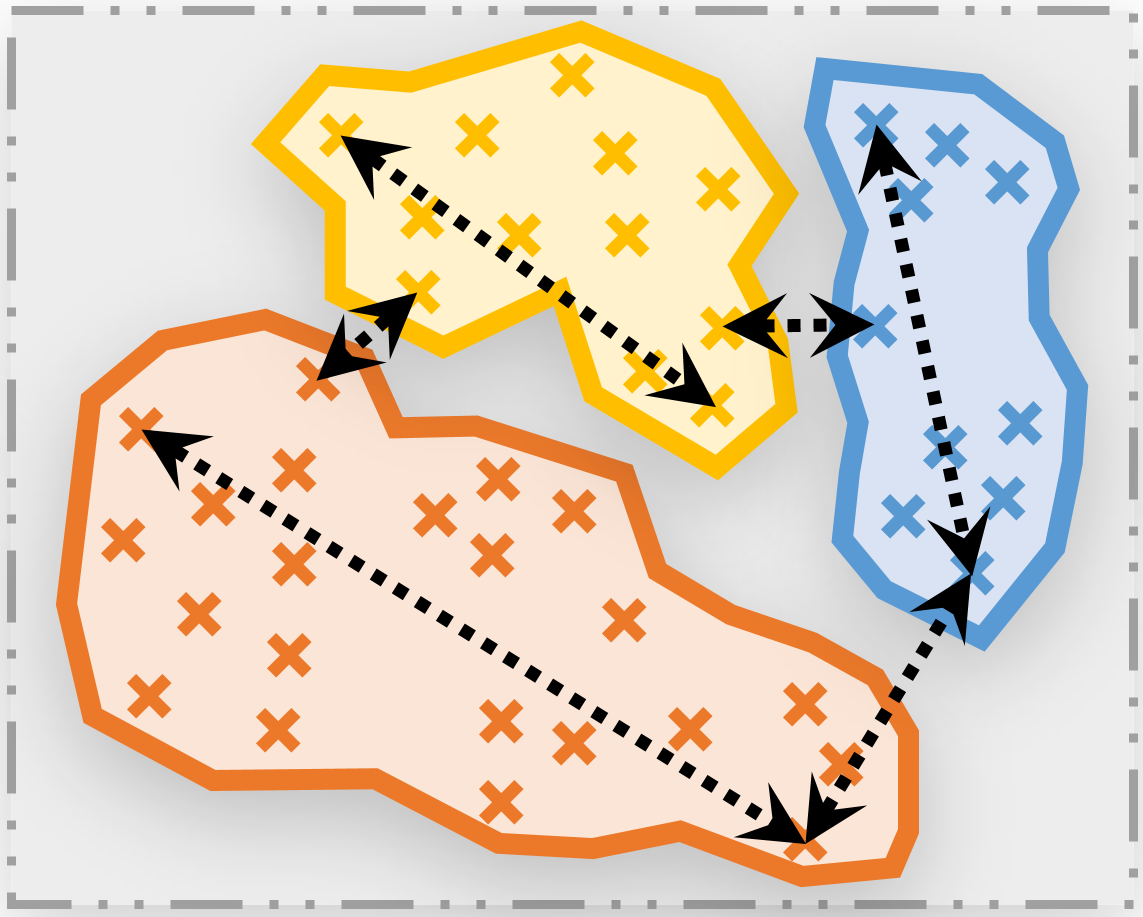
\includegraphics[width=0.35\textwidth]{figures/example-sampling}
			\caption{
				Exemples d'échantillonnages, sur la base de trois clusters, de données issues de mêmes clusters et étant les plus éloignées les unes des autres (\texttt{samp.farhtest.same}), et de données issues de clusters différents et étant les plus proches les unes des autres (\texttt{samp.closest.diff}).
			}
			\label{figure:3.3-CONTRAINTES-SAMPLING}
		\end{figure}

		Une classe abstraite définit les prérequis des algorithmes implémentés (avoir une méthode \texttt{sample}) et une \textit{factory} est disponible pour instancier rapidement un objet d'échantillonnage.
		% cognitivefactory.interactive-clustering.sampling : Exemple.
		Un exemple d'utilisation ce module est consultable dans \textsc{Code~\ref{code:3.3-IMPLEMENTATION-SAMPLING}}.
		
		\begin{lstlisting}[
			language=Python,
			caption={Démonstration de notre implémentation de l'échantillonnage sur le jeu d'exemple.},
			label={code:3.3-IMPLEMENTATION-SAMPLING},
		]
# Import des dépendances.
from cognitivefactory.interactive_clustering.sampling.factory import sampling_factory

# Initialiser un objet d'échantillonnage.
sampler = sampling_factory(
	algorithm="random",
	random_seed=42,
)

# Run sampling.
selection = sampler.sample(
	constraints_manager=constraints_manager,
	nb_to_select=2,
	clustering_result=clustering_result,  # optionnel pour "random"
	vectors=dict_of_vectors,  # optionnel pour "random"
)
"""
	[("0", '5"),  # "Comment signaler un vol de carte bancaire ?" vs "Le distributeur ne m'a pas rendu ma carte bleue."
	 ("0", '2"),  # "Comment signaler un vol de carte bancaire ?" vs "J'ai perdu ma carte de paiement"
	 ("2", 'N")]  # "J'ai perdu ma carte de paiement" vs "Pourquoi le sans contact ne fonctionne pas ?"
"""
		\end{lstlisting}
		

		%%%
		%%% Subsection 3.3.X:
		%%%
		\subsection{todo}
		\todo[inline]{SECTION À RÉDIGER: FMC}
		\todo[inline]{SECTION À RÉDIGER: IC-GUI page d'annotation}
		\todo[inline]{SECTION À RÉDIGER: IC-GUI gestion d'état de l'application}
		\todo[inline]{SECTION À RÉDIGER: IC-GUI page d'analyse (en cours)}

	
	%%%%%--------------------------------------------------------------------
	%%%%% Section 3.4:
	%%%%%--------------------------------------------------------------------
	\section{Espoirs de la méthode proposée}
		\todo[inline]{SECTION À RÉDIGER}

		•	Moins de formations, d'ateliers, …
		•	Se concentrer sur son domaine de compétence (i.e. pas de datascience pour les experts métiers)
		•	Permettre de trouver la base d'apprentissage
		•	Méthode réaliste / pas trop coûteuse
		•	…